% Created by tikzDevice version 0.7.0 on 2014-07-26 02:56:08
% !TEX encoding = UTF-8 Unicode
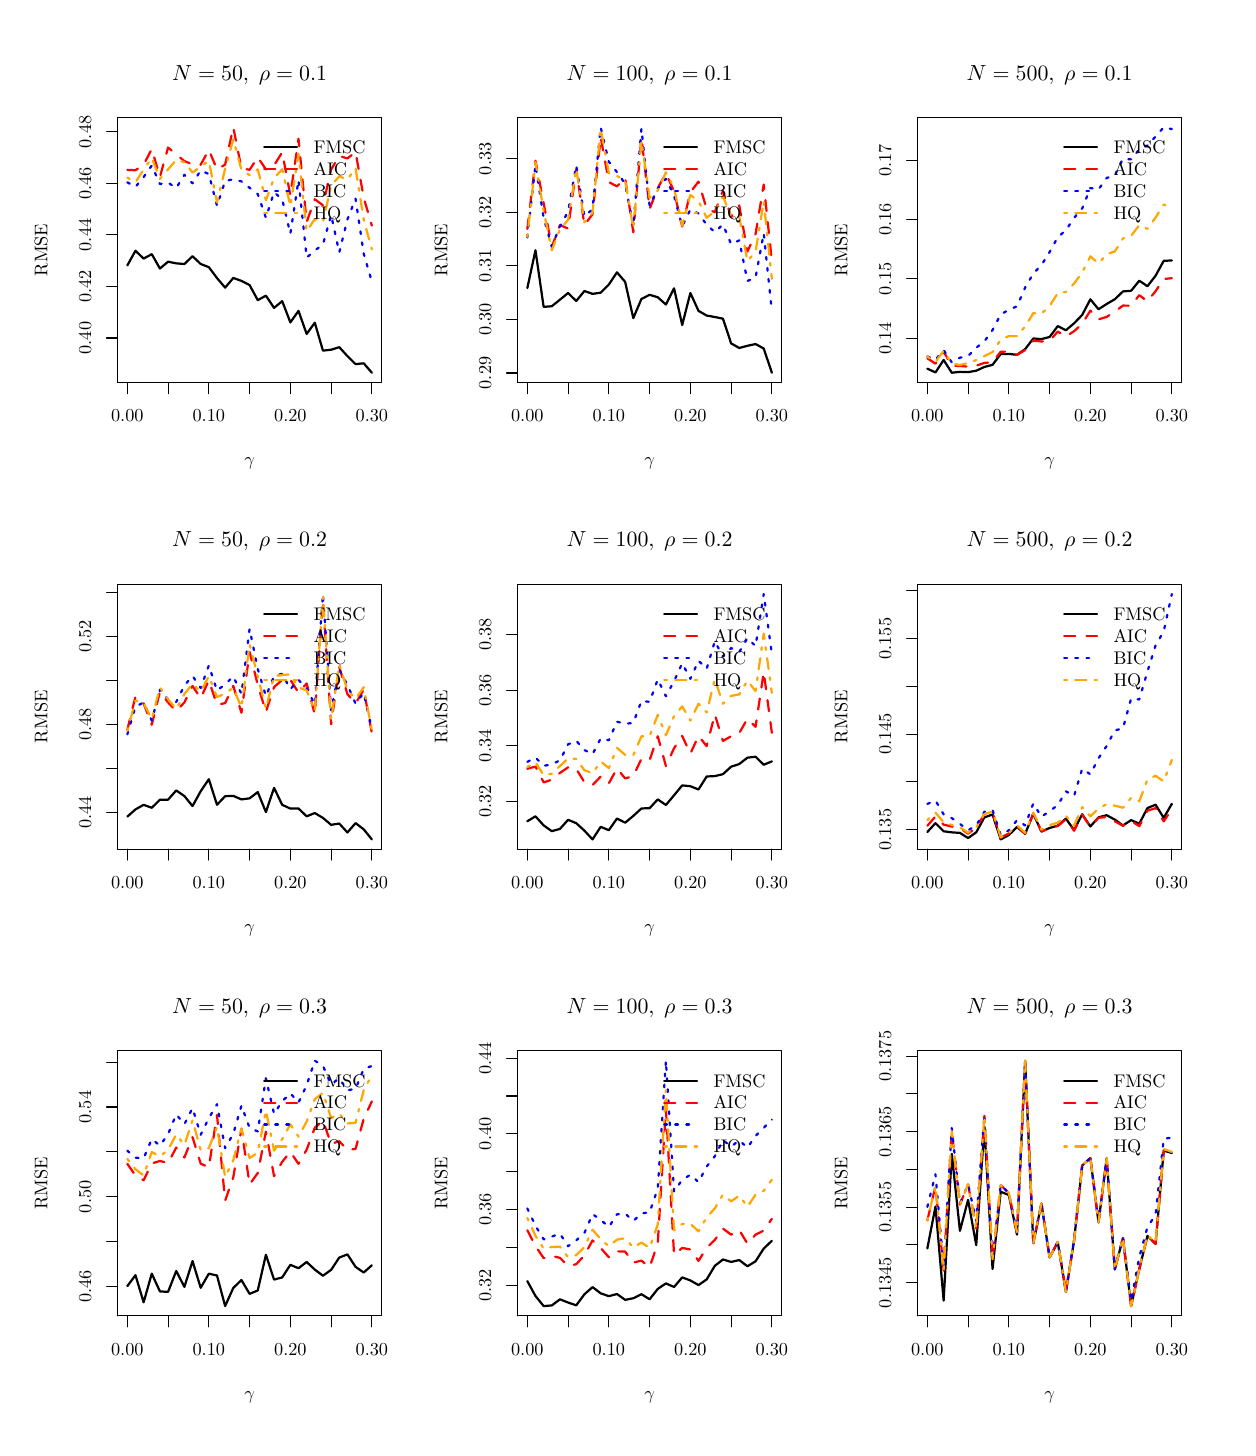
\begin{tikzpicture}[x=1pt,y=1pt]
\definecolor[named]{fillColor}{rgb}{1.00,1.00,1.00}
\path[use as bounding box,fill=fillColor,fill opacity=0.00] (0,0) rectangle (433.62,505.89);
\begin{scope}
\path[clip] ( 32.47,377.65) rectangle (127.91,473.42);
\definecolor[named]{drawColor}{rgb}{0.00,0.00,0.00}

\path[draw=drawColor,line width= 0.8pt,line join=round,line cap=round] ( 36.01,419.98) --
	( 38.95,425.27) --
	( 41.90,422.44) --
	( 44.84,424.05) --
	( 47.79,418.85) --
	( 50.73,421.31) --
	( 53.68,420.72) --
	( 56.63,420.48) --
	( 59.57,423.30) --
	( 62.52,420.49) --
	( 65.46,419.34) --
	( 68.41,415.41) --
	( 71.35,411.94) --
	( 74.30,415.44) --
	( 77.24,414.39) --
	( 80.19,412.88) --
	( 83.14,407.43) --
	( 86.08,409.04) --
	( 89.03,404.62) --
	( 91.97,407.07) --
	( 94.92,399.38) --
	( 97.86,403.54) --
	(100.81,395.21) --
	(103.75,399.27) --
	(106.70,389.18) --
	(109.65,389.51) --
	(112.59,390.43) --
	(115.54,387.21) --
	(118.48,384.31) --
	(121.43,384.60) --
	(124.37,381.20);
\end{scope}
\begin{scope}
\path[clip] (  0.00,  0.00) rectangle (433.62,505.89);
\definecolor[named]{drawColor}{rgb}{0.00,0.00,0.00}

\path[draw=drawColor,line width= 0.4pt,line join=round,line cap=round] ( 36.01,377.65) -- (124.37,377.65);

\path[draw=drawColor,line width= 0.4pt,line join=round,line cap=round] ( 36.01,377.65) -- ( 36.01,373.69);

\path[draw=drawColor,line width= 0.4pt,line join=round,line cap=round] ( 50.73,377.65) -- ( 50.73,373.69);

\path[draw=drawColor,line width= 0.4pt,line join=round,line cap=round] ( 65.46,377.65) -- ( 65.46,373.69);

\path[draw=drawColor,line width= 0.4pt,line join=round,line cap=round] ( 80.19,377.65) -- ( 80.19,373.69);

\path[draw=drawColor,line width= 0.4pt,line join=round,line cap=round] ( 94.92,377.65) -- ( 94.92,373.69);

\path[draw=drawColor,line width= 0.4pt,line join=round,line cap=round] (109.65,377.65) -- (109.65,373.69);

\path[draw=drawColor,line width= 0.4pt,line join=round,line cap=round] (124.37,377.65) -- (124.37,373.69);

\node[text=drawColor,anchor=base,inner sep=0pt, outer sep=0pt, scale=  0.66] at ( 36.01,363.40) {0.00};

\node[text=drawColor,anchor=base,inner sep=0pt, outer sep=0pt, scale=  0.66] at ( 65.46,363.40) {0.10};

\node[text=drawColor,anchor=base,inner sep=0pt, outer sep=0pt, scale=  0.66] at ( 94.92,363.40) {0.20};

\node[text=drawColor,anchor=base,inner sep=0pt, outer sep=0pt, scale=  0.66] at (124.37,363.40) {0.30};

\path[draw=drawColor,line width= 0.4pt,line join=round,line cap=round] ( 32.47,393.76) -- ( 32.47,468.22);

\path[draw=drawColor,line width= 0.4pt,line join=round,line cap=round] ( 32.47,393.76) -- ( 28.51,393.76);

\path[draw=drawColor,line width= 0.4pt,line join=round,line cap=round] ( 32.47,412.38) -- ( 28.51,412.38);

\path[draw=drawColor,line width= 0.4pt,line join=round,line cap=round] ( 32.47,430.99) -- ( 28.51,430.99);

\path[draw=drawColor,line width= 0.4pt,line join=round,line cap=round] ( 32.47,449.61) -- ( 28.51,449.61);

\path[draw=drawColor,line width= 0.4pt,line join=round,line cap=round] ( 32.47,468.22) -- ( 28.51,468.22);

\node[text=drawColor,rotate= 90.00,anchor=base,inner sep=0pt, outer sep=0pt, scale=  0.66] at ( 22.97,393.76) {0.40};

\node[text=drawColor,rotate= 90.00,anchor=base,inner sep=0pt, outer sep=0pt, scale=  0.66] at ( 22.97,412.38) {0.42};

\node[text=drawColor,rotate= 90.00,anchor=base,inner sep=0pt, outer sep=0pt, scale=  0.66] at ( 22.97,430.99) {0.44};

\node[text=drawColor,rotate= 90.00,anchor=base,inner sep=0pt, outer sep=0pt, scale=  0.66] at ( 22.97,449.61) {0.46};

\node[text=drawColor,rotate= 90.00,anchor=base,inner sep=0pt, outer sep=0pt, scale=  0.66] at ( 22.97,468.22) {0.48};

\path[draw=drawColor,line width= 0.4pt,line join=round,line cap=round] ( 32.47,377.65) --
	(127.91,377.65) --
	(127.91,473.42) --
	( 32.47,473.42) --
	( 32.47,377.65);
\end{scope}
\begin{scope}
\path[clip] (  0.00,337.26) rectangle (144.54,505.89);
\definecolor[named]{drawColor}{rgb}{0.00,0.00,0.00}

\node[text=drawColor,anchor=base,inner sep=0pt, outer sep=0pt, scale=  0.79] at ( 80.19,486.92) {\bfseries $N=50, \;\rho=0.1$};

\node[text=drawColor,anchor=base,inner sep=0pt, outer sep=0pt, scale=  0.66] at ( 80.19,347.56) {$\gamma$};

\node[text=drawColor,rotate= 90.00,anchor=base,inner sep=0pt, outer sep=0pt, scale=  0.66] at (  7.13,425.53) {RMSE};
\end{scope}
\begin{scope}
\path[clip] ( 32.47,377.65) rectangle (127.91,473.42);
\definecolor[named]{drawColor}{rgb}{1.00,0.00,0.00}

\path[draw=drawColor,line width= 0.8pt,dash pattern=on 4pt off 4pt ,line join=round,line cap=round] ( 36.01,454.51) --
	( 38.95,454.37) --
	( 41.90,456.37) --
	( 44.84,462.01) --
	( 47.79,451.98) --
	( 50.73,462.57) --
	( 53.68,460.13) --
	( 56.63,457.66) --
	( 59.57,456.51) --
	( 62.52,456.37) --
	( 65.46,461.75) --
	( 68.41,454.69) --
	( 71.35,456.41) --
	( 74.30,469.87) --
	( 77.24,455.12) --
	( 80.19,454.51) --
	( 83.14,459.05) --
	( 86.08,454.66) --
	( 89.03,456.14) --
	( 91.97,460.85) --
	( 94.92,445.26) --
	( 97.86,465.77) --
	(100.81,435.62) --
	(103.75,443.89) --
	(106.70,441.70) --
	(109.65,454.64) --
	(112.59,459.52) --
	(115.54,458.64) --
	(118.48,460.97) --
	(121.43,444.45) --
	(124.37,434.36);
\definecolor[named]{drawColor}{rgb}{0.00,0.00,1.00}

\path[draw=drawColor,line width= 0.8pt,dash pattern=on 1pt off 3pt ,line join=round,line cap=round] ( 36.01,450.00) --
	( 38.95,448.34) --
	( 41.90,451.92) --
	( 44.84,456.05) --
	( 47.79,449.39) --
	( 50.73,449.90) --
	( 53.68,447.96) --
	( 56.63,452.72) --
	( 59.57,449.66) --
	( 62.52,454.29) --
	( 65.46,452.99) --
	( 68.41,441.51) --
	( 71.35,450.47) --
	( 74.30,451.12) --
	( 77.24,450.33) --
	( 80.19,448.01) --
	( 83.14,445.74) --
	( 86.08,437.21) --
	( 89.03,446.41) --
	( 91.97,443.89) --
	( 94.92,431.44) --
	( 97.86,450.81) --
	(100.81,422.80) --
	(103.75,425.37) --
	(106.70,427.53) --
	(109.65,438.17) --
	(112.59,424.68) --
	(115.54,436.60) --
	(118.48,444.07) --
	(121.43,424.20) --
	(124.37,414.10);
\definecolor[named]{drawColor}{rgb}{1.00,0.65,0.00}

\path[draw=drawColor,line width= 0.8pt,dash pattern=on 1pt off 3pt on 4pt off 3pt ,line join=round,line cap=round] ( 36.01,451.68) --
	( 38.95,450.05) --
	( 41.90,454.57) --
	( 44.84,458.82) --
	( 47.79,451.26) --
	( 50.73,454.69) --
	( 53.68,458.09) --
	( 56.63,457.30) --
	( 59.57,453.55) --
	( 62.52,455.65) --
	( 65.46,457.78) --
	( 68.41,442.75) --
	( 71.35,454.91) --
	( 74.30,465.57) --
	( 77.24,454.56) --
	( 80.19,452.62) --
	( 83.14,454.67) --
	( 86.08,443.55) --
	( 89.03,451.54) --
	( 91.97,454.73) --
	( 94.92,441.34) --
	( 97.86,460.33) --
	(100.81,432.28) --
	(103.75,436.73) --
	(106.70,435.68) --
	(109.65,448.77) --
	(112.59,452.20) --
	(115.54,450.96) --
	(118.48,455.13) --
	(121.43,436.46) --
	(124.37,425.78);
\definecolor[named]{drawColor}{rgb}{0.00,0.00,0.00}

\path[draw=drawColor,line width= 0.8pt,line join=round,line cap=round] ( 85.47,462.63) -- ( 97.35,462.63);
\definecolor[named]{drawColor}{rgb}{1.00,0.00,0.00}

\path[draw=drawColor,line width= 0.8pt,dash pattern=on 4pt off 4pt ,line join=round,line cap=round] ( 85.47,454.71) -- ( 97.35,454.71);
\definecolor[named]{drawColor}{rgb}{0.00,0.00,1.00}

\path[draw=drawColor,line width= 0.8pt,dash pattern=on 1pt off 3pt ,line join=round,line cap=round] ( 85.47,446.79) -- ( 97.35,446.79);
\definecolor[named]{drawColor}{rgb}{1.00,0.65,0.00}

\path[draw=drawColor,line width= 0.8pt,dash pattern=on 1pt off 3pt on 4pt off 3pt ,line join=round,line cap=round] ( 85.47,438.87) -- ( 97.35,438.87);
\definecolor[named]{drawColor}{rgb}{0.00,0.00,0.00}

\node[text=drawColor,anchor=base west,inner sep=0pt, outer sep=0pt, scale=  0.66] at (103.29,460.35) {FMSC};

\node[text=drawColor,anchor=base west,inner sep=0pt, outer sep=0pt, scale=  0.66] at (103.29,452.43) {AIC};

\node[text=drawColor,anchor=base west,inner sep=0pt, outer sep=0pt, scale=  0.66] at (103.29,444.51) {BIC};

\node[text=drawColor,anchor=base west,inner sep=0pt, outer sep=0pt, scale=  0.66] at (103.29,436.59) {HQ};
\end{scope}
\begin{scope}
\path[clip] (177.01,377.65) rectangle (272.45,473.42);
\definecolor[named]{drawColor}{rgb}{0.00,0.00,0.00}

\path[draw=drawColor,line width= 0.8pt,line join=round,line cap=round] (180.55,411.78) --
	(183.49,425.46) --
	(186.44,405.00) --
	(189.38,405.22) --
	(192.33,407.58) --
	(195.27,410.01) --
	(198.22,407.12) --
	(201.17,410.72) --
	(204.11,409.70) --
	(207.06,410.12) --
	(210.00,413.07) --
	(212.95,417.47) --
	(215.89,414.03) --
	(218.84,400.94) --
	(221.78,407.85) --
	(224.73,409.36) --
	(227.68,408.47) --
	(230.62,405.84) --
	(233.57,411.69) --
	(236.51,398.44) --
	(239.46,410.02) --
	(242.40,403.55) --
	(245.35,401.86) --
	(248.29,401.34) --
	(251.24,400.73) --
	(254.19,391.79) --
	(257.13,390.14) --
	(260.08,390.93) --
	(263.02,391.57) --
	(265.97,389.94) --
	(268.91,381.20);
\end{scope}
\begin{scope}
\path[clip] (  0.00,  0.00) rectangle (433.62,505.89);
\definecolor[named]{drawColor}{rgb}{0.00,0.00,0.00}

\path[draw=drawColor,line width= 0.4pt,line join=round,line cap=round] (180.55,377.65) -- (268.91,377.65);

\path[draw=drawColor,line width= 0.4pt,line join=round,line cap=round] (180.55,377.65) -- (180.55,373.69);

\path[draw=drawColor,line width= 0.4pt,line join=round,line cap=round] (195.27,377.65) -- (195.27,373.69);

\path[draw=drawColor,line width= 0.4pt,line join=round,line cap=round] (210.00,377.65) -- (210.00,373.69);

\path[draw=drawColor,line width= 0.4pt,line join=round,line cap=round] (224.73,377.65) -- (224.73,373.69);

\path[draw=drawColor,line width= 0.4pt,line join=round,line cap=round] (239.46,377.65) -- (239.46,373.69);

\path[draw=drawColor,line width= 0.4pt,line join=round,line cap=round] (254.19,377.65) -- (254.19,373.69);

\path[draw=drawColor,line width= 0.4pt,line join=round,line cap=round] (268.91,377.65) -- (268.91,373.69);

\node[text=drawColor,anchor=base,inner sep=0pt, outer sep=0pt, scale=  0.66] at (180.55,363.40) {0.00};

\node[text=drawColor,anchor=base,inner sep=0pt, outer sep=0pt, scale=  0.66] at (210.00,363.40) {0.10};

\node[text=drawColor,anchor=base,inner sep=0pt, outer sep=0pt, scale=  0.66] at (239.46,363.40) {0.20};

\node[text=drawColor,anchor=base,inner sep=0pt, outer sep=0pt, scale=  0.66] at (268.91,363.40) {0.30};

\path[draw=drawColor,line width= 0.4pt,line join=round,line cap=round] (177.01,381.12) -- (177.01,458.51);

\path[draw=drawColor,line width= 0.4pt,line join=round,line cap=round] (177.01,381.12) -- (173.05,381.12);

\path[draw=drawColor,line width= 0.4pt,line join=round,line cap=round] (177.01,400.47) -- (173.05,400.47);

\path[draw=drawColor,line width= 0.4pt,line join=round,line cap=round] (177.01,419.82) -- (173.05,419.82);

\path[draw=drawColor,line width= 0.4pt,line join=round,line cap=round] (177.01,439.16) -- (173.05,439.16);

\path[draw=drawColor,line width= 0.4pt,line join=round,line cap=round] (177.01,458.51) -- (173.05,458.51);

\node[text=drawColor,rotate= 90.00,anchor=base,inner sep=0pt, outer sep=0pt, scale=  0.66] at (167.51,381.12) {0.29};

\node[text=drawColor,rotate= 90.00,anchor=base,inner sep=0pt, outer sep=0pt, scale=  0.66] at (167.51,400.47) {0.30};

\node[text=drawColor,rotate= 90.00,anchor=base,inner sep=0pt, outer sep=0pt, scale=  0.66] at (167.51,419.82) {0.31};

\node[text=drawColor,rotate= 90.00,anchor=base,inner sep=0pt, outer sep=0pt, scale=  0.66] at (167.51,439.16) {0.32};

\node[text=drawColor,rotate= 90.00,anchor=base,inner sep=0pt, outer sep=0pt, scale=  0.66] at (167.51,458.51) {0.33};

\path[draw=drawColor,line width= 0.4pt,line join=round,line cap=round] (177.01,377.65) --
	(272.45,377.65) --
	(272.45,473.42) --
	(177.01,473.42) --
	(177.01,377.65);
\end{scope}
\begin{scope}
\path[clip] (144.54,337.26) rectangle (289.08,505.89);
\definecolor[named]{drawColor}{rgb}{0.00,0.00,0.00}

\node[text=drawColor,anchor=base,inner sep=0pt, outer sep=0pt, scale=  0.79] at (224.73,486.92) {\bfseries $N=100, \;\rho=0.1$};

\node[text=drawColor,anchor=base,inner sep=0pt, outer sep=0pt, scale=  0.66] at (224.73,347.56) {$\gamma$};

\node[text=drawColor,rotate= 90.00,anchor=base,inner sep=0pt, outer sep=0pt, scale=  0.66] at (151.67,425.53) {RMSE};
\end{scope}
\begin{scope}
\path[clip] (177.01,377.65) rectangle (272.45,473.42);
\definecolor[named]{drawColor}{rgb}{1.00,0.00,0.00}

\path[draw=drawColor,line width= 0.8pt,dash pattern=on 4pt off 4pt ,line join=round,line cap=round] (180.55,433.13) --
	(183.49,457.79) --
	(186.44,442.51) --
	(189.38,426.62) --
	(192.33,434.56) --
	(195.27,433.30) --
	(198.22,454.75) --
	(201.17,434.59) --
	(204.11,438.45) --
	(207.06,466.31) --
	(210.00,450.11) --
	(212.95,448.53) --
	(215.89,451.57) --
	(218.84,431.93) --
	(221.78,466.25) --
	(224.73,440.37) --
	(227.68,447.93) --
	(230.62,453.28) --
	(233.57,446.73) --
	(236.51,434.04) --
	(239.46,446.43) --
	(242.40,450.26) --
	(245.35,440.39) --
	(248.29,439.23) --
	(251.24,446.99) --
	(254.19,437.47) --
	(257.13,441.64) --
	(260.08,425.00) --
	(263.02,431.33) --
	(265.97,449.21) --
	(268.91,421.60);
\definecolor[named]{drawColor}{rgb}{0.00,0.00,1.00}

\path[draw=drawColor,line width= 0.8pt,dash pattern=on 1pt off 3pt ,line join=round,line cap=round] (180.55,430.08) --
	(183.49,456.31) --
	(186.44,437.16) --
	(189.38,426.89) --
	(192.33,434.01) --
	(195.27,439.44) --
	(198.22,456.10) --
	(201.17,437.72) --
	(204.11,440.28) --
	(207.06,469.87) --
	(210.00,457.42) --
	(212.95,453.67) --
	(215.89,449.48) --
	(218.84,434.16) --
	(221.78,469.42) --
	(224.73,441.53) --
	(227.68,447.80) --
	(230.62,451.28) --
	(233.57,445.13) --
	(236.51,434.10) --
	(239.46,440.18) --
	(242.40,438.74) --
	(245.35,434.67) --
	(248.29,432.00) --
	(251.24,434.77) --
	(254.19,427.65) --
	(257.13,429.02) --
	(260.08,414.35) --
	(263.02,415.57) --
	(265.97,431.59) --
	(268.91,403.38);
\definecolor[named]{drawColor}{rgb}{1.00,0.65,0.00}

\path[draw=drawColor,line width= 0.8pt,dash pattern=on 1pt off 3pt on 4pt off 3pt ,line join=round,line cap=round] (180.55,430.34) --
	(183.49,457.30) --
	(186.44,439.72) --
	(189.38,425.47) --
	(192.33,433.03) --
	(195.27,436.42) --
	(198.22,454.90) --
	(201.17,435.60) --
	(204.11,438.97) --
	(207.06,469.44) --
	(210.00,453.35) --
	(212.95,452.27) --
	(215.89,450.78) --
	(218.84,433.35) --
	(221.78,464.97) --
	(224.73,444.43) --
	(227.68,447.03) --
	(230.62,453.63) --
	(233.57,448.02) --
	(236.51,434.30) --
	(239.46,445.43) --
	(242.40,443.20) --
	(245.35,437.19) --
	(248.29,439.56) --
	(251.24,444.90) --
	(254.19,437.73) --
	(257.13,437.59) --
	(260.08,421.56) --
	(263.02,424.89) --
	(265.97,443.14) --
	(268.91,415.12);
\definecolor[named]{drawColor}{rgb}{0.00,0.00,0.00}

\path[draw=drawColor,line width= 0.8pt,line join=round,line cap=round] (230.01,462.63) -- (241.89,462.63);
\definecolor[named]{drawColor}{rgb}{1.00,0.00,0.00}

\path[draw=drawColor,line width= 0.8pt,dash pattern=on 4pt off 4pt ,line join=round,line cap=round] (230.01,454.71) -- (241.89,454.71);
\definecolor[named]{drawColor}{rgb}{0.00,0.00,1.00}

\path[draw=drawColor,line width= 0.8pt,dash pattern=on 1pt off 3pt ,line join=round,line cap=round] (230.01,446.79) -- (241.89,446.79);
\definecolor[named]{drawColor}{rgb}{1.00,0.65,0.00}

\path[draw=drawColor,line width= 0.8pt,dash pattern=on 1pt off 3pt on 4pt off 3pt ,line join=round,line cap=round] (230.01,438.87) -- (241.89,438.87);
\definecolor[named]{drawColor}{rgb}{0.00,0.00,0.00}

\node[text=drawColor,anchor=base west,inner sep=0pt, outer sep=0pt, scale=  0.66] at (247.83,460.35) {FMSC};

\node[text=drawColor,anchor=base west,inner sep=0pt, outer sep=0pt, scale=  0.66] at (247.83,452.43) {AIC};

\node[text=drawColor,anchor=base west,inner sep=0pt, outer sep=0pt, scale=  0.66] at (247.83,444.51) {BIC};

\node[text=drawColor,anchor=base west,inner sep=0pt, outer sep=0pt, scale=  0.66] at (247.83,436.59) {HQ};
\end{scope}
\begin{scope}
\path[clip] (321.55,377.65) rectangle (416.99,473.42);
\definecolor[named]{drawColor}{rgb}{0.00,0.00,0.00}

\path[draw=drawColor,line width= 0.8pt,line join=round,line cap=round] (325.09,382.67) --
	(328.03,381.30) --
	(330.98,385.80) --
	(333.92,381.20) --
	(336.87,381.52) --
	(339.81,381.41) --
	(342.76,381.93) --
	(345.71,383.29) --
	(348.65,384.05) --
	(351.60,387.95) --
	(354.54,387.99) --
	(357.49,387.68) --
	(360.43,389.72) --
	(363.38,393.58) --
	(366.32,393.35) --
	(369.27,394.12) --
	(372.22,398.06) --
	(375.16,396.55) --
	(378.11,399.05) --
	(381.05,402.09) --
	(384.00,407.73) --
	(386.94,404.14) --
	(389.89,406.03) --
	(392.83,407.75) --
	(395.78,410.58) --
	(398.73,410.81) --
	(401.67,414.44) --
	(404.62,412.46) --
	(407.56,416.24) --
	(410.51,421.64) --
	(413.45,421.76);
\end{scope}
\begin{scope}
\path[clip] (  0.00,  0.00) rectangle (433.62,505.89);
\definecolor[named]{drawColor}{rgb}{0.00,0.00,0.00}

\path[draw=drawColor,line width= 0.4pt,line join=round,line cap=round] (325.09,377.65) -- (413.45,377.65);

\path[draw=drawColor,line width= 0.4pt,line join=round,line cap=round] (325.09,377.65) -- (325.09,373.69);

\path[draw=drawColor,line width= 0.4pt,line join=round,line cap=round] (339.81,377.65) -- (339.81,373.69);

\path[draw=drawColor,line width= 0.4pt,line join=round,line cap=round] (354.54,377.65) -- (354.54,373.69);

\path[draw=drawColor,line width= 0.4pt,line join=round,line cap=round] (369.27,377.65) -- (369.27,373.69);

\path[draw=drawColor,line width= 0.4pt,line join=round,line cap=round] (384.00,377.65) -- (384.00,373.69);

\path[draw=drawColor,line width= 0.4pt,line join=round,line cap=round] (398.73,377.65) -- (398.73,373.69);

\path[draw=drawColor,line width= 0.4pt,line join=round,line cap=round] (413.45,377.65) -- (413.45,373.69);

\node[text=drawColor,anchor=base,inner sep=0pt, outer sep=0pt, scale=  0.66] at (325.09,363.40) {0.00};

\node[text=drawColor,anchor=base,inner sep=0pt, outer sep=0pt, scale=  0.66] at (354.54,363.40) {0.10};

\node[text=drawColor,anchor=base,inner sep=0pt, outer sep=0pt, scale=  0.66] at (384.00,363.40) {0.20};

\node[text=drawColor,anchor=base,inner sep=0pt, outer sep=0pt, scale=  0.66] at (413.45,363.40) {0.30};

\path[draw=drawColor,line width= 0.4pt,line join=round,line cap=round] (321.55,393.69) -- (321.55,457.97);

\path[draw=drawColor,line width= 0.4pt,line join=round,line cap=round] (321.55,393.69) -- (317.59,393.69);

\path[draw=drawColor,line width= 0.4pt,line join=round,line cap=round] (321.55,415.12) -- (317.59,415.12);

\path[draw=drawColor,line width= 0.4pt,line join=round,line cap=round] (321.55,436.54) -- (317.59,436.54);

\path[draw=drawColor,line width= 0.4pt,line join=round,line cap=round] (321.55,457.97) -- (317.59,457.97);

\node[text=drawColor,rotate= 90.00,anchor=base,inner sep=0pt, outer sep=0pt, scale=  0.66] at (312.05,393.69) {0.14};

\node[text=drawColor,rotate= 90.00,anchor=base,inner sep=0pt, outer sep=0pt, scale=  0.66] at (312.05,415.12) {0.15};

\node[text=drawColor,rotate= 90.00,anchor=base,inner sep=0pt, outer sep=0pt, scale=  0.66] at (312.05,436.54) {0.16};

\node[text=drawColor,rotate= 90.00,anchor=base,inner sep=0pt, outer sep=0pt, scale=  0.66] at (312.05,457.97) {0.17};

\path[draw=drawColor,line width= 0.4pt,line join=round,line cap=round] (321.55,377.65) --
	(416.99,377.65) --
	(416.99,473.42) --
	(321.55,473.42) --
	(321.55,377.65);
\end{scope}
\begin{scope}
\path[clip] (289.08,337.26) rectangle (433.62,505.89);
\definecolor[named]{drawColor}{rgb}{0.00,0.00,0.00}

\node[text=drawColor,anchor=base,inner sep=0pt, outer sep=0pt, scale=  0.79] at (369.27,486.92) {\bfseries $N=500, \;\rho=0.1$};

\node[text=drawColor,anchor=base,inner sep=0pt, outer sep=0pt, scale=  0.66] at (369.27,347.56) {$\gamma$};

\node[text=drawColor,rotate= 90.00,anchor=base,inner sep=0pt, outer sep=0pt, scale=  0.66] at (296.21,425.53) {RMSE};
\end{scope}
\begin{scope}
\path[clip] (321.55,377.65) rectangle (416.99,473.42);
\definecolor[named]{drawColor}{rgb}{1.00,0.00,0.00}

\path[draw=drawColor,line width= 0.8pt,dash pattern=on 4pt off 4pt ,line join=round,line cap=round] (325.09,386.42) --
	(328.03,384.47) --
	(330.98,388.83) --
	(333.92,383.72) --
	(336.87,383.64) --
	(339.81,383.40) --
	(342.76,383.74) --
	(345.71,384.76) --
	(348.65,384.99) --
	(351.60,388.78) --
	(354.54,388.87) --
	(357.49,387.66) --
	(360.43,389.38) --
	(363.38,392.79) --
	(366.32,392.49) --
	(369.27,392.73) --
	(372.22,396.08) --
	(375.16,394.27) --
	(378.11,396.20) --
	(381.05,398.89) --
	(384.00,403.64) --
	(386.94,400.49) --
	(389.89,401.37) --
	(392.83,403.26) --
	(395.78,405.46) --
	(398.73,405.43) --
	(401.67,409.23) --
	(404.62,407.03) --
	(407.56,410.67) --
	(410.51,415.06) --
	(413.45,415.36);
\definecolor[named]{drawColor}{rgb}{0.00,0.00,1.00}

\path[draw=drawColor,line width= 0.8pt,dash pattern=on 1pt off 3pt ,line join=round,line cap=round] (325.09,387.09) --
	(328.03,385.88) --
	(330.98,389.35) --
	(333.92,384.97) --
	(336.87,386.64) --
	(339.81,387.21) --
	(342.76,390.24) --
	(345.71,392.54) --
	(348.65,396.61) --
	(351.60,402.28) --
	(354.54,403.92) --
	(357.49,405.21) --
	(360.43,411.99) --
	(363.38,417.01) --
	(366.32,420.09) --
	(369.27,424.80) --
	(372.22,430.16) --
	(375.16,432.70) --
	(378.11,437.14) --
	(381.05,440.58) --
	(384.00,447.96) --
	(386.94,447.41) --
	(389.89,451.57) --
	(392.83,452.57) --
	(395.78,458.54) --
	(398.73,458.29) --
	(401.67,461.90) --
	(404.62,463.34) --
	(407.56,466.55) --
	(410.51,469.87) --
	(413.45,469.25);
\definecolor[named]{drawColor}{rgb}{1.00,0.65,0.00}

\path[draw=drawColor,line width= 0.8pt,dash pattern=on 1pt off 3pt on 4pt off 3pt ,line join=round,line cap=round] (325.09,387.04) --
	(328.03,385.19) --
	(330.98,389.08) --
	(333.92,384.51) --
	(336.87,383.99) --
	(339.81,384.74) --
	(342.76,385.77) --
	(345.71,387.19) --
	(348.65,388.65) --
	(351.60,393.15) --
	(354.54,394.44) --
	(357.49,394.42) --
	(360.43,397.94) --
	(363.38,402.75) --
	(366.32,402.51) --
	(369.27,405.36) --
	(372.22,409.96) --
	(375.16,410.39) --
	(378.11,413.43) --
	(381.05,417.44) --
	(384.00,423.26) --
	(386.94,420.65) --
	(389.89,424.02) --
	(392.83,425.02) --
	(395.78,429.74) --
	(398.73,430.68) --
	(401.67,434.54) --
	(404.62,433.20) --
	(407.56,437.27) --
	(410.51,441.98) --
	(413.45,440.84);
\definecolor[named]{drawColor}{rgb}{0.00,0.00,0.00}

\path[draw=drawColor,line width= 0.8pt,line join=round,line cap=round] (374.55,462.63) -- (386.43,462.63);
\definecolor[named]{drawColor}{rgb}{1.00,0.00,0.00}

\path[draw=drawColor,line width= 0.8pt,dash pattern=on 4pt off 4pt ,line join=round,line cap=round] (374.55,454.71) -- (386.43,454.71);
\definecolor[named]{drawColor}{rgb}{0.00,0.00,1.00}

\path[draw=drawColor,line width= 0.8pt,dash pattern=on 1pt off 3pt ,line join=round,line cap=round] (374.55,446.79) -- (386.43,446.79);
\definecolor[named]{drawColor}{rgb}{1.00,0.65,0.00}

\path[draw=drawColor,line width= 0.8pt,dash pattern=on 1pt off 3pt on 4pt off 3pt ,line join=round,line cap=round] (374.55,438.87) -- (386.43,438.87);
\definecolor[named]{drawColor}{rgb}{0.00,0.00,0.00}

\node[text=drawColor,anchor=base west,inner sep=0pt, outer sep=0pt, scale=  0.66] at (392.37,460.35) {FMSC};

\node[text=drawColor,anchor=base west,inner sep=0pt, outer sep=0pt, scale=  0.66] at (392.37,452.43) {AIC};

\node[text=drawColor,anchor=base west,inner sep=0pt, outer sep=0pt, scale=  0.66] at (392.37,444.51) {BIC};

\node[text=drawColor,anchor=base west,inner sep=0pt, outer sep=0pt, scale=  0.66] at (392.37,436.59) {HQ};
\end{scope}
\begin{scope}
\path[clip] ( 32.47,209.02) rectangle (127.91,304.79);
\definecolor[named]{drawColor}{rgb}{0.00,0.00,0.00}

\path[draw=drawColor,line width= 0.8pt,line join=round,line cap=round] ( 36.01,220.79) --
	( 38.95,223.41) --
	( 41.90,225.06) --
	( 44.84,224.00) --
	( 47.79,226.90) --
	( 50.73,226.92) --
	( 53.68,230.27) --
	( 56.63,228.23) --
	( 59.57,224.62) --
	( 62.52,229.97) --
	( 65.46,234.33) --
	( 68.41,225.08) --
	( 71.35,228.18) --
	( 74.30,228.29) --
	( 77.24,227.02) --
	( 80.19,227.41) --
	( 83.14,229.66) --
	( 86.08,222.44) --
	( 89.03,231.19) --
	( 91.97,225.06) --
	( 94.92,223.71) --
	( 97.86,223.74) --
	(100.81,220.91) --
	(103.75,222.10) --
	(106.70,220.33) --
	(109.65,217.84) --
	(112.59,218.30) --
	(115.54,215.08) --
	(118.48,218.46) --
	(121.43,216.20) --
	(124.37,212.57);
\end{scope}
\begin{scope}
\path[clip] (  0.00,  0.00) rectangle (433.62,505.89);
\definecolor[named]{drawColor}{rgb}{0.00,0.00,0.00}

\path[draw=drawColor,line width= 0.4pt,line join=round,line cap=round] ( 36.01,209.02) -- (124.37,209.02);

\path[draw=drawColor,line width= 0.4pt,line join=round,line cap=round] ( 36.01,209.02) -- ( 36.01,205.06);

\path[draw=drawColor,line width= 0.4pt,line join=round,line cap=round] ( 50.73,209.02) -- ( 50.73,205.06);

\path[draw=drawColor,line width= 0.4pt,line join=round,line cap=round] ( 65.46,209.02) -- ( 65.46,205.06);

\path[draw=drawColor,line width= 0.4pt,line join=round,line cap=round] ( 80.19,209.02) -- ( 80.19,205.06);

\path[draw=drawColor,line width= 0.4pt,line join=round,line cap=round] ( 94.92,209.02) -- ( 94.92,205.06);

\path[draw=drawColor,line width= 0.4pt,line join=round,line cap=round] (109.65,209.02) -- (109.65,205.06);

\path[draw=drawColor,line width= 0.4pt,line join=round,line cap=round] (124.37,209.02) -- (124.37,205.06);

\node[text=drawColor,anchor=base,inner sep=0pt, outer sep=0pt, scale=  0.66] at ( 36.01,194.77) {0.00};

\node[text=drawColor,anchor=base,inner sep=0pt, outer sep=0pt, scale=  0.66] at ( 65.46,194.77) {0.10};

\node[text=drawColor,anchor=base,inner sep=0pt, outer sep=0pt, scale=  0.66] at ( 94.92,194.77) {0.20};

\node[text=drawColor,anchor=base,inner sep=0pt, outer sep=0pt, scale=  0.66] at (124.37,194.77) {0.30};

\path[draw=drawColor,line width= 0.4pt,line join=round,line cap=round] ( 32.47,222.43) -- ( 32.47,301.79);

\path[draw=drawColor,line width= 0.4pt,line join=round,line cap=round] ( 32.47,222.43) -- ( 28.51,222.43);

\path[draw=drawColor,line width= 0.4pt,line join=round,line cap=round] ( 32.47,238.31) -- ( 28.51,238.31);

\path[draw=drawColor,line width= 0.4pt,line join=round,line cap=round] ( 32.47,254.18) -- ( 28.51,254.18);

\path[draw=drawColor,line width= 0.4pt,line join=round,line cap=round] ( 32.47,270.05) -- ( 28.51,270.05);

\path[draw=drawColor,line width= 0.4pt,line join=round,line cap=round] ( 32.47,285.92) -- ( 28.51,285.92);

\path[draw=drawColor,line width= 0.4pt,line join=round,line cap=round] ( 32.47,301.79) -- ( 28.51,301.79);

\node[text=drawColor,rotate= 90.00,anchor=base,inner sep=0pt, outer sep=0pt, scale=  0.66] at ( 22.97,222.43) {0.44};

\node[text=drawColor,rotate= 90.00,anchor=base,inner sep=0pt, outer sep=0pt, scale=  0.66] at ( 22.97,254.18) {0.48};

\node[text=drawColor,rotate= 90.00,anchor=base,inner sep=0pt, outer sep=0pt, scale=  0.66] at ( 22.97,285.92) {0.52};

\path[draw=drawColor,line width= 0.4pt,line join=round,line cap=round] ( 32.47,209.02) --
	(127.91,209.02) --
	(127.91,304.79) --
	( 32.47,304.79) --
	( 32.47,209.02);
\end{scope}
\begin{scope}
\path[clip] (  0.00,168.63) rectangle (144.54,337.26);
\definecolor[named]{drawColor}{rgb}{0.00,0.00,0.00}

\node[text=drawColor,anchor=base,inner sep=0pt, outer sep=0pt, scale=  0.79] at ( 80.19,318.29) {\bfseries $N=50, \;\rho=0.2$};

\node[text=drawColor,anchor=base,inner sep=0pt, outer sep=0pt, scale=  0.66] at ( 80.19,178.93) {$\gamma$};

\node[text=drawColor,rotate= 90.00,anchor=base,inner sep=0pt, outer sep=0pt, scale=  0.66] at (  7.13,256.90) {RMSE};
\end{scope}
\begin{scope}
\path[clip] ( 32.47,209.02) rectangle (127.91,304.79);
\definecolor[named]{drawColor}{rgb}{1.00,0.00,0.00}

\path[draw=drawColor,line width= 0.8pt,dash pattern=on 4pt off 4pt ,line join=round,line cap=round] ( 36.01,252.16) --
	( 38.95,264.14) --
	( 41.90,261.70) --
	( 44.84,254.01) --
	( 47.79,265.90) --
	( 50.73,262.05) --
	( 53.68,258.91) --
	( 56.63,262.06) --
	( 59.57,268.00) --
	( 62.52,263.57) --
	( 65.46,270.07) --
	( 68.41,261.22) --
	( 71.35,261.81) --
	( 74.30,268.05) --
	( 77.24,258.33) --
	( 80.19,280.32) --
	( 83.14,268.38) --
	( 86.08,258.66) --
	( 89.03,267.60) --
	( 91.97,270.21) --
	( 94.92,270.28) --
	( 97.86,265.58) --
	(100.81,268.91) --
	(103.75,257.74) --
	(106.70,298.93) --
	(109.65,254.19) --
	(112.59,274.87) --
	(115.54,265.06) --
	(118.48,261.70) --
	(121.43,266.70) --
	(124.37,251.04);
\definecolor[named]{drawColor}{rgb}{0.00,0.00,1.00}

\path[draw=drawColor,line width= 0.8pt,dash pattern=on 1pt off 3pt ,line join=round,line cap=round] ( 36.01,250.52) --
	( 38.95,260.56) --
	( 41.90,262.02) --
	( 44.84,255.49) --
	( 47.79,266.65) --
	( 50.73,263.17) --
	( 53.68,262.21) --
	( 56.63,268.16) --
	( 59.57,271.63) --
	( 62.52,267.29) --
	( 65.46,275.42) --
	( 68.41,266.38) --
	( 71.35,268.60) --
	( 74.30,271.48) --
	( 77.24,265.14) --
	( 80.19,288.63) --
	( 83.14,274.14) --
	( 86.08,264.33) --
	( 89.03,271.57) --
	( 91.97,272.44) --
	( 94.92,266.84) --
	( 97.86,270.20) --
	(100.81,267.18) --
	(103.75,261.29) --
	(106.70,301.24) --
	(109.65,259.25) --
	(112.59,273.85) --
	(115.54,268.44) --
	(118.48,261.63) --
	(121.43,265.51) --
	(124.37,252.31);
\definecolor[named]{drawColor}{rgb}{1.00,0.65,0.00}

\path[draw=drawColor,line width= 0.8pt,dash pattern=on 1pt off 3pt on 4pt off 3pt ,line join=round,line cap=round] ( 36.01,251.82) --
	( 38.95,262.74) --
	( 41.90,261.75) --
	( 44.84,256.08) --
	( 47.79,267.49) --
	( 50.73,263.20) --
	( 53.68,259.60) --
	( 56.63,265.13) --
	( 59.57,268.75) --
	( 62.52,265.98) --
	( 65.46,271.61) --
	( 68.41,263.95) --
	( 71.35,265.36) --
	( 74.30,267.34) --
	( 77.24,260.19) --
	( 80.19,283.12) --
	( 83.14,271.44) --
	( 86.08,259.84) --
	( 89.03,271.54) --
	( 91.97,271.99) --
	( 94.92,272.20) --
	( 97.86,267.47) --
	(100.81,266.41) --
	(103.75,258.91) --
	(106.70,300.24) --
	(109.65,255.85) --
	(112.59,275.86) --
	(115.54,266.48) --
	(118.48,263.38) --
	(121.43,267.54) --
	(124.37,251.94);
\definecolor[named]{drawColor}{rgb}{0.00,0.00,0.00}

\path[draw=drawColor,line width= 0.8pt,line join=round,line cap=round] ( 85.47,294.00) -- ( 97.35,294.00);
\definecolor[named]{drawColor}{rgb}{1.00,0.00,0.00}

\path[draw=drawColor,line width= 0.8pt,dash pattern=on 4pt off 4pt ,line join=round,line cap=round] ( 85.47,286.08) -- ( 97.35,286.08);
\definecolor[named]{drawColor}{rgb}{0.00,0.00,1.00}

\path[draw=drawColor,line width= 0.8pt,dash pattern=on 1pt off 3pt ,line join=round,line cap=round] ( 85.47,278.16) -- ( 97.35,278.16);
\definecolor[named]{drawColor}{rgb}{1.00,0.65,0.00}

\path[draw=drawColor,line width= 0.8pt,dash pattern=on 1pt off 3pt on 4pt off 3pt ,line join=round,line cap=round] ( 85.47,270.24) -- ( 97.35,270.24);
\definecolor[named]{drawColor}{rgb}{0.00,0.00,0.00}

\node[text=drawColor,anchor=base west,inner sep=0pt, outer sep=0pt, scale=  0.66] at (103.29,291.72) {FMSC};

\node[text=drawColor,anchor=base west,inner sep=0pt, outer sep=0pt, scale=  0.66] at (103.29,283.80) {AIC};

\node[text=drawColor,anchor=base west,inner sep=0pt, outer sep=0pt, scale=  0.66] at (103.29,275.88) {BIC};

\node[text=drawColor,anchor=base west,inner sep=0pt, outer sep=0pt, scale=  0.66] at (103.29,267.96) {HQ};
\end{scope}
\begin{scope}
\path[clip] (177.01,209.02) rectangle (272.45,304.79);
\definecolor[named]{drawColor}{rgb}{0.00,0.00,0.00}

\path[draw=drawColor,line width= 0.8pt,line join=round,line cap=round] (180.55,219.14) --
	(183.49,220.91) --
	(186.44,217.64) --
	(189.38,215.55) --
	(192.33,216.35) --
	(195.27,219.65) --
	(198.22,218.43) --
	(201.17,215.73) --
	(204.11,212.57) --
	(207.06,217.11) --
	(210.00,215.90) --
	(212.95,220.11) --
	(215.89,218.60) --
	(218.84,221.05) --
	(221.78,223.75) --
	(224.73,223.85) --
	(227.68,227.03) --
	(230.62,225.00) --
	(233.57,228.51) --
	(236.51,232.08) --
	(239.46,231.79) --
	(242.40,230.61) --
	(245.35,235.30) --
	(248.29,235.44) --
	(251.24,236.14) --
	(254.19,238.84) --
	(257.13,239.81) --
	(260.08,242.10) --
	(263.02,242.44) --
	(265.97,239.54) --
	(268.91,240.76);
\end{scope}
\begin{scope}
\path[clip] (  0.00,  0.00) rectangle (433.62,505.89);
\definecolor[named]{drawColor}{rgb}{0.00,0.00,0.00}

\path[draw=drawColor,line width= 0.4pt,line join=round,line cap=round] (180.55,209.02) -- (268.91,209.02);

\path[draw=drawColor,line width= 0.4pt,line join=round,line cap=round] (180.55,209.02) -- (180.55,205.06);

\path[draw=drawColor,line width= 0.4pt,line join=round,line cap=round] (195.27,209.02) -- (195.27,205.06);

\path[draw=drawColor,line width= 0.4pt,line join=round,line cap=round] (210.00,209.02) -- (210.00,205.06);

\path[draw=drawColor,line width= 0.4pt,line join=round,line cap=round] (224.73,209.02) -- (224.73,205.06);

\path[draw=drawColor,line width= 0.4pt,line join=round,line cap=round] (239.46,209.02) -- (239.46,205.06);

\path[draw=drawColor,line width= 0.4pt,line join=round,line cap=round] (254.19,209.02) -- (254.19,205.06);

\path[draw=drawColor,line width= 0.4pt,line join=round,line cap=round] (268.91,209.02) -- (268.91,205.06);

\node[text=drawColor,anchor=base,inner sep=0pt, outer sep=0pt, scale=  0.66] at (180.55,194.77) {0.00};

\node[text=drawColor,anchor=base,inner sep=0pt, outer sep=0pt, scale=  0.66] at (210.00,194.77) {0.10};

\node[text=drawColor,anchor=base,inner sep=0pt, outer sep=0pt, scale=  0.66] at (239.46,194.77) {0.20};

\node[text=drawColor,anchor=base,inner sep=0pt, outer sep=0pt, scale=  0.66] at (268.91,194.77) {0.30};

\path[draw=drawColor,line width= 0.4pt,line join=round,line cap=round] (177.01,226.27) -- (177.01,286.56);

\path[draw=drawColor,line width= 0.4pt,line join=round,line cap=round] (177.01,226.27) -- (173.05,226.27);

\path[draw=drawColor,line width= 0.4pt,line join=round,line cap=round] (177.01,246.37) -- (173.05,246.37);

\path[draw=drawColor,line width= 0.4pt,line join=round,line cap=round] (177.01,266.46) -- (173.05,266.46);

\path[draw=drawColor,line width= 0.4pt,line join=round,line cap=round] (177.01,286.56) -- (173.05,286.56);

\node[text=drawColor,rotate= 90.00,anchor=base,inner sep=0pt, outer sep=0pt, scale=  0.66] at (167.51,226.27) {0.32};

\node[text=drawColor,rotate= 90.00,anchor=base,inner sep=0pt, outer sep=0pt, scale=  0.66] at (167.51,246.37) {0.34};

\node[text=drawColor,rotate= 90.00,anchor=base,inner sep=0pt, outer sep=0pt, scale=  0.66] at (167.51,266.46) {0.36};

\node[text=drawColor,rotate= 90.00,anchor=base,inner sep=0pt, outer sep=0pt, scale=  0.66] at (167.51,286.56) {0.38};

\path[draw=drawColor,line width= 0.4pt,line join=round,line cap=round] (177.01,209.02) --
	(272.45,209.02) --
	(272.45,304.79) --
	(177.01,304.79) --
	(177.01,209.02);
\end{scope}
\begin{scope}
\path[clip] (144.54,168.63) rectangle (289.08,337.26);
\definecolor[named]{drawColor}{rgb}{0.00,0.00,0.00}

\node[text=drawColor,anchor=base,inner sep=0pt, outer sep=0pt, scale=  0.79] at (224.73,318.29) {\bfseries $N=100, \;\rho=0.2$};

\node[text=drawColor,anchor=base,inner sep=0pt, outer sep=0pt, scale=  0.66] at (224.73,178.93) {$\gamma$};

\node[text=drawColor,rotate= 90.00,anchor=base,inner sep=0pt, outer sep=0pt, scale=  0.66] at (151.67,256.90) {RMSE};
\end{scope}
\begin{scope}
\path[clip] (177.01,209.02) rectangle (272.45,304.79);
\definecolor[named]{drawColor}{rgb}{1.00,0.00,0.00}

\path[draw=drawColor,line width= 0.8pt,dash pattern=on 4pt off 4pt ,line join=round,line cap=round] (180.55,238.08) --
	(183.49,238.88) --
	(186.44,233.17) --
	(189.38,234.15) --
	(192.33,236.59) --
	(195.27,238.59) --
	(198.22,238.08) --
	(201.17,233.21) --
	(204.11,232.20) --
	(207.06,235.29) --
	(210.00,232.84) --
	(212.95,238.19) --
	(215.89,234.62) --
	(218.84,235.44) --
	(221.78,241.70) --
	(224.73,241.21) --
	(227.68,249.84) --
	(230.62,239.11) --
	(233.57,245.51) --
	(236.51,249.95) --
	(239.46,243.56) --
	(242.40,249.96) --
	(245.35,246.26) --
	(248.29,257.74) --
	(251.24,248.12) --
	(254.19,249.87) --
	(257.13,250.97) --
	(260.08,256.20) --
	(263.02,253.24) --
	(265.97,273.08) --
	(268.91,251.07);
\definecolor[named]{drawColor}{rgb}{0.00,0.00,1.00}

\path[draw=drawColor,line width= 0.8pt,dash pattern=on 1pt off 3pt ,line join=round,line cap=round] (180.55,240.59) --
	(183.49,242.12) --
	(186.44,239.18) --
	(189.38,239.63) --
	(192.33,241.18) --
	(195.27,246.90) --
	(198.22,248.21) --
	(201.17,244.85) --
	(204.11,243.39) --
	(207.06,249.05) --
	(210.00,248.41) --
	(212.95,255.10) --
	(215.89,254.33) --
	(218.84,254.68) --
	(221.78,262.59) --
	(224.73,262.27) --
	(227.68,270.39) --
	(230.62,264.31) --
	(233.57,269.76) --
	(236.51,276.21) --
	(239.46,270.60) --
	(242.40,277.12) --
	(245.35,274.22) --
	(248.29,284.18) --
	(251.24,278.64) --
	(254.19,281.71) --
	(257.13,280.28) --
	(260.08,285.29) --
	(263.02,282.41) --
	(265.97,301.24) --
	(268.91,279.52);
\definecolor[named]{drawColor}{rgb}{1.00,0.65,0.00}

\path[draw=drawColor,line width= 0.8pt,dash pattern=on 1pt off 3pt on 4pt off 3pt ,line join=round,line cap=round] (180.55,238.69) --
	(183.49,240.45) --
	(186.44,235.79) --
	(189.38,236.31) --
	(192.33,239.08) --
	(195.27,241.86) --
	(198.22,241.66) --
	(201.17,237.57) --
	(204.11,236.47) --
	(207.06,240.74) --
	(210.00,238.32) --
	(212.95,245.65) --
	(215.89,243.12) --
	(218.84,243.01) --
	(221.78,249.82) --
	(224.73,249.90) --
	(227.68,257.59) --
	(230.62,250.17) --
	(233.57,257.14) --
	(236.51,260.65) --
	(239.46,255.50) --
	(242.40,261.60) --
	(245.35,258.46) --
	(248.29,270.45) --
	(251.24,261.61) --
	(254.19,264.44) --
	(257.13,264.96) --
	(260.08,269.96) --
	(263.02,266.15) --
	(265.97,286.98) --
	(268.91,265.52);
\definecolor[named]{drawColor}{rgb}{0.00,0.00,0.00}

\path[draw=drawColor,line width= 0.8pt,line join=round,line cap=round] (230.01,294.00) -- (241.89,294.00);
\definecolor[named]{drawColor}{rgb}{1.00,0.00,0.00}

\path[draw=drawColor,line width= 0.8pt,dash pattern=on 4pt off 4pt ,line join=round,line cap=round] (230.01,286.08) -- (241.89,286.08);
\definecolor[named]{drawColor}{rgb}{0.00,0.00,1.00}

\path[draw=drawColor,line width= 0.8pt,dash pattern=on 1pt off 3pt ,line join=round,line cap=round] (230.01,278.16) -- (241.89,278.16);
\definecolor[named]{drawColor}{rgb}{1.00,0.65,0.00}

\path[draw=drawColor,line width= 0.8pt,dash pattern=on 1pt off 3pt on 4pt off 3pt ,line join=round,line cap=round] (230.01,270.24) -- (241.89,270.24);
\definecolor[named]{drawColor}{rgb}{0.00,0.00,0.00}

\node[text=drawColor,anchor=base west,inner sep=0pt, outer sep=0pt, scale=  0.66] at (247.83,291.72) {FMSC};

\node[text=drawColor,anchor=base west,inner sep=0pt, outer sep=0pt, scale=  0.66] at (247.83,283.80) {AIC};

\node[text=drawColor,anchor=base west,inner sep=0pt, outer sep=0pt, scale=  0.66] at (247.83,275.88) {BIC};

\node[text=drawColor,anchor=base west,inner sep=0pt, outer sep=0pt, scale=  0.66] at (247.83,267.96) {HQ};
\end{scope}
\begin{scope}
\path[clip] (321.55,209.02) rectangle (416.99,304.79);
\definecolor[named]{drawColor}{rgb}{0.00,0.00,0.00}

\path[draw=drawColor,line width= 0.8pt,line join=round,line cap=round] (325.09,215.24) --
	(328.03,218.44) --
	(330.98,215.50) --
	(333.92,215.12) --
	(336.87,214.92) --
	(339.81,213.05) --
	(342.76,215.13) --
	(345.71,220.55) --
	(348.65,221.55) --
	(351.60,212.57) --
	(354.54,214.14) --
	(357.49,217.04) --
	(360.43,214.56) --
	(363.38,221.82) --
	(366.32,215.38) --
	(369.27,216.70) --
	(372.22,217.53) --
	(375.16,220.08) --
	(378.11,215.95) --
	(381.05,221.67) --
	(384.00,217.25) --
	(386.94,220.54) --
	(389.89,221.31) --
	(392.83,219.72) --
	(395.78,217.61) --
	(398.73,219.54) --
	(401.67,218.23) --
	(404.62,223.89) --
	(407.56,225.11) --
	(410.51,220.35) --
	(413.45,225.43);
\end{scope}
\begin{scope}
\path[clip] (  0.00,  0.00) rectangle (433.62,505.89);
\definecolor[named]{drawColor}{rgb}{0.00,0.00,0.00}

\path[draw=drawColor,line width= 0.4pt,line join=round,line cap=round] (325.09,209.02) -- (413.45,209.02);

\path[draw=drawColor,line width= 0.4pt,line join=round,line cap=round] (325.09,209.02) -- (325.09,205.06);

\path[draw=drawColor,line width= 0.4pt,line join=round,line cap=round] (339.81,209.02) -- (339.81,205.06);

\path[draw=drawColor,line width= 0.4pt,line join=round,line cap=round] (354.54,209.02) -- (354.54,205.06);

\path[draw=drawColor,line width= 0.4pt,line join=round,line cap=round] (369.27,209.02) -- (369.27,205.06);

\path[draw=drawColor,line width= 0.4pt,line join=round,line cap=round] (384.00,209.02) -- (384.00,205.06);

\path[draw=drawColor,line width= 0.4pt,line join=round,line cap=round] (398.73,209.02) -- (398.73,205.06);

\path[draw=drawColor,line width= 0.4pt,line join=round,line cap=round] (413.45,209.02) -- (413.45,205.06);

\node[text=drawColor,anchor=base,inner sep=0pt, outer sep=0pt, scale=  0.66] at (325.09,194.77) {0.00};

\node[text=drawColor,anchor=base,inner sep=0pt, outer sep=0pt, scale=  0.66] at (354.54,194.77) {0.10};

\node[text=drawColor,anchor=base,inner sep=0pt, outer sep=0pt, scale=  0.66] at (384.00,194.77) {0.20};

\node[text=drawColor,anchor=base,inner sep=0pt, outer sep=0pt, scale=  0.66] at (413.45,194.77) {0.30};

\path[draw=drawColor,line width= 0.4pt,line join=round,line cap=round] (321.55,216.10) -- (321.55,302.40);

\path[draw=drawColor,line width= 0.4pt,line join=round,line cap=round] (321.55,216.10) -- (317.59,216.10);

\path[draw=drawColor,line width= 0.4pt,line join=round,line cap=round] (321.55,233.36) -- (317.59,233.36);

\path[draw=drawColor,line width= 0.4pt,line join=round,line cap=round] (321.55,250.62) -- (317.59,250.62);

\path[draw=drawColor,line width= 0.4pt,line join=round,line cap=round] (321.55,267.88) -- (317.59,267.88);

\path[draw=drawColor,line width= 0.4pt,line join=round,line cap=round] (321.55,285.14) -- (317.59,285.14);

\path[draw=drawColor,line width= 0.4pt,line join=round,line cap=round] (321.55,302.40) -- (317.59,302.40);

\node[text=drawColor,rotate= 90.00,anchor=base,inner sep=0pt, outer sep=0pt, scale=  0.66] at (312.05,216.10) {0.135};

\node[text=drawColor,rotate= 90.00,anchor=base,inner sep=0pt, outer sep=0pt, scale=  0.66] at (312.05,250.62) {0.145};

\node[text=drawColor,rotate= 90.00,anchor=base,inner sep=0pt, outer sep=0pt, scale=  0.66] at (312.05,285.14) {0.155};

\path[draw=drawColor,line width= 0.4pt,line join=round,line cap=round] (321.55,209.02) --
	(416.99,209.02) --
	(416.99,304.79) --
	(321.55,304.79) --
	(321.55,209.02);
\end{scope}
\begin{scope}
\path[clip] (289.08,168.63) rectangle (433.62,337.26);
\definecolor[named]{drawColor}{rgb}{0.00,0.00,0.00}

\node[text=drawColor,anchor=base,inner sep=0pt, outer sep=0pt, scale=  0.79] at (369.27,318.29) {\bfseries $N=500, \;\rho=0.2$};

\node[text=drawColor,anchor=base,inner sep=0pt, outer sep=0pt, scale=  0.66] at (369.27,178.93) {$\gamma$};

\node[text=drawColor,rotate= 90.00,anchor=base,inner sep=0pt, outer sep=0pt, scale=  0.66] at (296.21,256.90) {RMSE};
\end{scope}
\begin{scope}
\path[clip] (321.55,209.02) rectangle (416.99,304.79);
\definecolor[named]{drawColor}{rgb}{1.00,0.00,0.00}

\path[draw=drawColor,line width= 0.8pt,dash pattern=on 4pt off 4pt ,line join=round,line cap=round] (325.09,217.49) --
	(328.03,220.85) --
	(330.98,217.90) --
	(333.92,217.21) --
	(336.87,216.61) --
	(339.81,214.66) --
	(342.76,216.75) --
	(345.71,221.68) --
	(348.65,222.41) --
	(351.60,213.22) --
	(354.54,214.72) --
	(357.49,217.28) --
	(360.43,214.65) --
	(363.38,222.00) --
	(366.32,215.45) --
	(369.27,216.69) --
	(372.22,217.41) --
	(375.16,219.86) --
	(378.11,215.70) --
	(381.05,221.47) --
	(384.00,217.15) --
	(386.94,220.38) --
	(389.89,220.65) --
	(392.83,219.12) --
	(395.78,217.48) --
	(398.73,219.21) --
	(401.67,217.39) --
	(404.62,222.94) --
	(407.56,223.87) --
	(410.51,219.08) --
	(413.45,223.48);
\definecolor[named]{drawColor}{rgb}{0.00,0.00,1.00}

\path[draw=drawColor,line width= 0.8pt,dash pattern=on 1pt off 3pt ,line join=round,line cap=round] (325.09,225.39) --
	(328.03,226.59) --
	(330.98,221.61) --
	(333.92,220.25) --
	(336.87,218.17) --
	(339.81,215.86) --
	(342.76,217.62) --
	(345.71,222.57) --
	(348.65,223.17) --
	(351.60,214.12) --
	(354.54,215.85) --
	(357.49,219.50) --
	(360.43,217.63) --
	(363.38,225.55) --
	(366.32,220.72) --
	(369.27,222.82) --
	(372.22,224.92) --
	(375.16,229.95) --
	(378.11,228.26) --
	(381.05,238.09) --
	(384.00,236.08) --
	(386.94,241.88) --
	(389.89,246.34) --
	(392.83,251.94) --
	(395.78,252.71) --
	(398.73,263.49) --
	(401.67,263.13) --
	(404.62,273.18) --
	(407.56,282.66) --
	(410.51,287.77) --
	(413.45,301.24);
\definecolor[named]{drawColor}{rgb}{1.00,0.65,0.00}

\path[draw=drawColor,line width= 0.8pt,dash pattern=on 1pt off 3pt on 4pt off 3pt ,line join=round,line cap=round] (325.09,219.54) --
	(328.03,222.24) --
	(330.98,218.77) --
	(333.92,217.77) --
	(336.87,216.95) --
	(339.81,214.98) --
	(342.76,216.96) --
	(345.71,221.75) --
	(348.65,222.64) --
	(351.60,213.29) --
	(354.54,214.92) --
	(357.49,217.68) --
	(360.43,214.94) --
	(363.38,222.28) --
	(366.32,216.14) --
	(369.27,217.73) --
	(372.22,218.63) --
	(375.16,221.12) --
	(378.11,217.61) --
	(381.05,224.24) --
	(384.00,220.91) --
	(386.94,223.74) --
	(389.89,225.29) --
	(392.83,224.78) --
	(395.78,224.01) --
	(398.73,227.62) --
	(401.67,226.34) --
	(404.62,234.18) --
	(407.56,235.57) --
	(410.51,233.53) --
	(413.45,241.32);
\definecolor[named]{drawColor}{rgb}{0.00,0.00,0.00}

\path[draw=drawColor,line width= 0.8pt,line join=round,line cap=round] (374.55,294.00) -- (386.43,294.00);
\definecolor[named]{drawColor}{rgb}{1.00,0.00,0.00}

\path[draw=drawColor,line width= 0.8pt,dash pattern=on 4pt off 4pt ,line join=round,line cap=round] (374.55,286.08) -- (386.43,286.08);
\definecolor[named]{drawColor}{rgb}{0.00,0.00,1.00}

\path[draw=drawColor,line width= 0.8pt,dash pattern=on 1pt off 3pt ,line join=round,line cap=round] (374.55,278.16) -- (386.43,278.16);
\definecolor[named]{drawColor}{rgb}{1.00,0.65,0.00}

\path[draw=drawColor,line width= 0.8pt,dash pattern=on 1pt off 3pt on 4pt off 3pt ,line join=round,line cap=round] (374.55,270.24) -- (386.43,270.24);
\definecolor[named]{drawColor}{rgb}{0.00,0.00,0.00}

\node[text=drawColor,anchor=base west,inner sep=0pt, outer sep=0pt, scale=  0.66] at (392.37,291.72) {FMSC};

\node[text=drawColor,anchor=base west,inner sep=0pt, outer sep=0pt, scale=  0.66] at (392.37,283.80) {AIC};

\node[text=drawColor,anchor=base west,inner sep=0pt, outer sep=0pt, scale=  0.66] at (392.37,275.88) {BIC};

\node[text=drawColor,anchor=base west,inner sep=0pt, outer sep=0pt, scale=  0.66] at (392.37,267.96) {HQ};
\end{scope}
\begin{scope}
\path[clip] ( 32.47, 40.39) rectangle (127.91,136.16);
\definecolor[named]{drawColor}{rgb}{0.00,0.00,0.00}

\path[draw=drawColor,line width= 0.8pt,line join=round,line cap=round] ( 36.01, 51.14) --
	( 38.95, 55.10) --
	( 41.90, 45.30) --
	( 44.84, 55.65) --
	( 47.79, 49.24) --
	( 50.73, 49.06) --
	( 53.68, 56.62) --
	( 56.63, 50.88) --
	( 59.57, 60.21) --
	( 62.52, 50.54) --
	( 65.46, 55.64) --
	( 68.41, 54.99) --
	( 71.35, 43.94) --
	( 74.30, 50.49) --
	( 77.24, 53.34) --
	( 80.19, 48.36) --
	( 83.14, 49.57) --
	( 86.08, 62.47) --
	( 89.03, 53.52) --
	( 91.97, 54.28) --
	( 94.92, 58.84) --
	( 97.86, 57.62) --
	(100.81, 59.87) --
	(103.75, 57.12) --
	(106.70, 54.91) --
	(109.65, 57.03) --
	(112.59, 61.46) --
	(115.54, 62.63) --
	(118.48, 58.11) --
	(121.43, 56.07) --
	(124.37, 58.68);
\end{scope}
\begin{scope}
\path[clip] (  0.00,  0.00) rectangle (433.62,505.89);
\definecolor[named]{drawColor}{rgb}{0.00,0.00,0.00}

\path[draw=drawColor,line width= 0.4pt,line join=round,line cap=round] ( 36.01, 40.39) -- (124.37, 40.39);

\path[draw=drawColor,line width= 0.4pt,line join=round,line cap=round] ( 36.01, 40.39) -- ( 36.01, 36.43);

\path[draw=drawColor,line width= 0.4pt,line join=round,line cap=round] ( 50.73, 40.39) -- ( 50.73, 36.43);

\path[draw=drawColor,line width= 0.4pt,line join=round,line cap=round] ( 65.46, 40.39) -- ( 65.46, 36.43);

\path[draw=drawColor,line width= 0.4pt,line join=round,line cap=round] ( 80.19, 40.39) -- ( 80.19, 36.43);

\path[draw=drawColor,line width= 0.4pt,line join=round,line cap=round] ( 94.92, 40.39) -- ( 94.92, 36.43);

\path[draw=drawColor,line width= 0.4pt,line join=round,line cap=round] (109.65, 40.39) -- (109.65, 36.43);

\path[draw=drawColor,line width= 0.4pt,line join=round,line cap=round] (124.37, 40.39) -- (124.37, 36.43);

\node[text=drawColor,anchor=base,inner sep=0pt, outer sep=0pt, scale=  0.66] at ( 36.01, 26.14) {0.00};

\node[text=drawColor,anchor=base,inner sep=0pt, outer sep=0pt, scale=  0.66] at ( 65.46, 26.14) {0.10};

\node[text=drawColor,anchor=base,inner sep=0pt, outer sep=0pt, scale=  0.66] at ( 94.92, 26.14) {0.20};

\node[text=drawColor,anchor=base,inner sep=0pt, outer sep=0pt, scale=  0.66] at (124.37, 26.14) {0.30};

\path[draw=drawColor,line width= 0.4pt,line join=round,line cap=round] ( 32.47, 50.99) -- ( 32.47,132.09);

\path[draw=drawColor,line width= 0.4pt,line join=round,line cap=round] ( 32.47, 50.99) -- ( 28.51, 50.99);

\path[draw=drawColor,line width= 0.4pt,line join=round,line cap=round] ( 32.47, 67.21) -- ( 28.51, 67.21);

\path[draw=drawColor,line width= 0.4pt,line join=round,line cap=round] ( 32.47, 83.43) -- ( 28.51, 83.43);

\path[draw=drawColor,line width= 0.4pt,line join=round,line cap=round] ( 32.47, 99.65) -- ( 28.51, 99.65);

\path[draw=drawColor,line width= 0.4pt,line join=round,line cap=round] ( 32.47,115.87) -- ( 28.51,115.87);

\path[draw=drawColor,line width= 0.4pt,line join=round,line cap=round] ( 32.47,132.09) -- ( 28.51,132.09);

\node[text=drawColor,rotate= 90.00,anchor=base,inner sep=0pt, outer sep=0pt, scale=  0.66] at ( 22.97, 50.99) {0.46};

\node[text=drawColor,rotate= 90.00,anchor=base,inner sep=0pt, outer sep=0pt, scale=  0.66] at ( 22.97, 83.43) {0.50};

\node[text=drawColor,rotate= 90.00,anchor=base,inner sep=0pt, outer sep=0pt, scale=  0.66] at ( 22.97,115.87) {0.54};

\path[draw=drawColor,line width= 0.4pt,line join=round,line cap=round] ( 32.47, 40.39) --
	(127.91, 40.39) --
	(127.91,136.16) --
	( 32.47,136.16) --
	( 32.47, 40.39);
\end{scope}
\begin{scope}
\path[clip] (  0.00,  0.00) rectangle (144.54,168.63);
\definecolor[named]{drawColor}{rgb}{0.00,0.00,0.00}

\node[text=drawColor,anchor=base,inner sep=0pt, outer sep=0pt, scale=  0.79] at ( 80.19,149.66) {\bfseries $N=50, \;\rho=0.3$};

\node[text=drawColor,anchor=base,inner sep=0pt, outer sep=0pt, scale=  0.66] at ( 80.19, 10.30) {$\gamma$};

\node[text=drawColor,rotate= 90.00,anchor=base,inner sep=0pt, outer sep=0pt, scale=  0.66] at (  7.13, 88.27) {RMSE};
\end{scope}
\begin{scope}
\path[clip] ( 32.47, 40.39) rectangle (127.91,136.16);
\definecolor[named]{drawColor}{rgb}{1.00,0.00,0.00}

\path[draw=drawColor,line width= 0.8pt,dash pattern=on 4pt off 4pt ,line join=round,line cap=round] ( 36.01, 95.34) --
	( 38.95, 91.11) --
	( 41.90, 89.42) --
	( 44.84, 95.49) --
	( 47.79, 96.36) --
	( 50.73, 95.64) --
	( 53.68,101.21) --
	( 56.63, 97.64) --
	( 59.57,104.98) --
	( 62.52, 95.40) --
	( 65.46, 94.08) --
	( 68.41,113.00) --
	( 71.35, 82.02) --
	( 74.30, 90.51) --
	( 77.24,108.01) --
	( 80.19, 87.91) --
	( 83.14, 92.00) --
	( 86.08,106.97) --
	( 89.03, 90.86) --
	( 91.97, 96.08) --
	( 94.92, 99.69) --
	( 97.86, 95.32) --
	(100.81,100.44) --
	(103.75,108.38) --
	(106.70,111.01) --
	(109.65,102.51) --
	(112.59,103.52) --
	(115.54,100.32) --
	(118.48,100.74) --
	(121.43,111.64) --
	(124.37,117.91);
\definecolor[named]{drawColor}{rgb}{0.00,0.00,1.00}

\path[draw=drawColor,line width= 0.8pt,dash pattern=on 1pt off 3pt ,line join=round,line cap=round] ( 36.01,100.09) --
	( 38.95, 97.55) --
	( 41.90, 97.36) --
	( 44.84,104.27) --
	( 47.79,101.92) --
	( 50.73,106.05) --
	( 53.68,113.19) --
	( 56.63,109.66) --
	( 59.57,115.46) --
	( 62.52,105.86) --
	( 65.46,111.84) --
	( 68.41,116.87) --
	( 71.35,101.02) --
	( 74.30,106.20) --
	( 77.24,116.36) --
	( 80.19,108.32) --
	( 83.14,107.04) --
	( 86.08,126.28) --
	( 89.03,113.40) --
	( 91.97,117.95) --
	( 94.92,120.83) --
	( 97.86,117.51) --
	(100.81,123.76) --
	(103.75,132.61) --
	(106.70,130.72) --
	(109.65,124.12) --
	(112.59,126.21) --
	(115.54,121.91) --
	(118.48,122.48) --
	(121.43,129.62) --
	(124.37,130.70);
\definecolor[named]{drawColor}{rgb}{1.00,0.65,0.00}

\path[draw=drawColor,line width= 0.8pt,dash pattern=on 1pt off 3pt on 4pt off 3pt ,line join=round,line cap=round] ( 36.01, 97.11) --
	( 38.95, 93.37) --
	( 41.90, 91.15) --
	( 44.84, 99.60) --
	( 47.79, 98.02) --
	( 50.73,100.40) --
	( 53.68,105.96) --
	( 56.63,102.13) --
	( 59.57,111.07) --
	( 62.52,100.30) --
	( 65.46,101.02) --
	( 68.41,108.66) --
	( 71.35, 90.54) --
	( 74.30, 96.63) --
	( 77.24,108.12) --
	( 80.19, 97.44) --
	( 83.14, 99.38) --
	( 86.08,114.63) --
	( 89.03,100.11) --
	( 91.97,104.27) --
	( 94.92,109.60) --
	( 97.86,105.17) --
	(100.81,110.62) --
	(103.75,118.73) --
	(106.70,120.96) --
	(109.65,111.89) --
	(112.59,113.48) --
	(115.54,109.93) --
	(118.48,110.19) --
	(121.43,121.98) --
	(124.37,127.40);
\definecolor[named]{drawColor}{rgb}{0.00,0.00,0.00}

\path[draw=drawColor,line width= 0.8pt,line join=round,line cap=round] ( 85.47,125.37) -- ( 97.35,125.37);
\definecolor[named]{drawColor}{rgb}{1.00,0.00,0.00}

\path[draw=drawColor,line width= 0.8pt,dash pattern=on 4pt off 4pt ,line join=round,line cap=round] ( 85.47,117.45) -- ( 97.35,117.45);
\definecolor[named]{drawColor}{rgb}{0.00,0.00,1.00}

\path[draw=drawColor,line width= 0.8pt,dash pattern=on 1pt off 3pt ,line join=round,line cap=round] ( 85.47,109.53) -- ( 97.35,109.53);
\definecolor[named]{drawColor}{rgb}{1.00,0.65,0.00}

\path[draw=drawColor,line width= 0.8pt,dash pattern=on 1pt off 3pt on 4pt off 3pt ,line join=round,line cap=round] ( 85.47,101.61) -- ( 97.35,101.61);
\definecolor[named]{drawColor}{rgb}{0.00,0.00,0.00}

\node[text=drawColor,anchor=base west,inner sep=0pt, outer sep=0pt, scale=  0.66] at (103.29,123.09) {FMSC};

\node[text=drawColor,anchor=base west,inner sep=0pt, outer sep=0pt, scale=  0.66] at (103.29,115.17) {AIC};

\node[text=drawColor,anchor=base west,inner sep=0pt, outer sep=0pt, scale=  0.66] at (103.29,107.25) {BIC};

\node[text=drawColor,anchor=base west,inner sep=0pt, outer sep=0pt, scale=  0.66] at (103.29, 99.33) {HQ};
\end{scope}
\begin{scope}
\path[clip] (177.01, 40.39) rectangle (272.45,136.16);
\definecolor[named]{drawColor}{rgb}{0.00,0.00,0.00}

\path[draw=drawColor,line width= 0.8pt,line join=round,line cap=round] (180.55, 52.96) --
	(183.49, 47.59) --
	(186.44, 43.94) --
	(189.38, 44.17) --
	(192.33, 46.38) --
	(195.27, 45.22) --
	(198.22, 44.20) --
	(201.17, 48.19) --
	(204.11, 50.79) --
	(207.06, 48.55) --
	(210.00, 47.52) --
	(212.95, 48.29) --
	(215.89, 46.19) --
	(218.84, 46.77) --
	(221.78, 48.23) --
	(224.73, 46.38) --
	(227.68, 50.14) --
	(230.62, 52.13) --
	(233.57, 50.84) --
	(236.51, 54.30) --
	(239.46, 53.20) --
	(242.40, 51.53) --
	(245.35, 53.57) --
	(248.29, 58.47) --
	(251.24, 60.79) --
	(254.19, 59.89) --
	(257.13, 60.56) --
	(260.08, 58.31) --
	(263.02, 60.12) --
	(265.97, 64.72) --
	(268.91, 67.53);
\end{scope}
\begin{scope}
\path[clip] (  0.00,  0.00) rectangle (433.62,505.89);
\definecolor[named]{drawColor}{rgb}{0.00,0.00,0.00}

\path[draw=drawColor,line width= 0.4pt,line join=round,line cap=round] (180.55, 40.39) -- (268.91, 40.39);

\path[draw=drawColor,line width= 0.4pt,line join=round,line cap=round] (180.55, 40.39) -- (180.55, 36.43);

\path[draw=drawColor,line width= 0.4pt,line join=round,line cap=round] (195.27, 40.39) -- (195.27, 36.43);

\path[draw=drawColor,line width= 0.4pt,line join=round,line cap=round] (210.00, 40.39) -- (210.00, 36.43);

\path[draw=drawColor,line width= 0.4pt,line join=round,line cap=round] (224.73, 40.39) -- (224.73, 36.43);

\path[draw=drawColor,line width= 0.4pt,line join=round,line cap=round] (239.46, 40.39) -- (239.46, 36.43);

\path[draw=drawColor,line width= 0.4pt,line join=round,line cap=round] (254.19, 40.39) -- (254.19, 36.43);

\path[draw=drawColor,line width= 0.4pt,line join=round,line cap=round] (268.91, 40.39) -- (268.91, 36.43);

\node[text=drawColor,anchor=base,inner sep=0pt, outer sep=0pt, scale=  0.66] at (180.55, 26.14) {0.00};

\node[text=drawColor,anchor=base,inner sep=0pt, outer sep=0pt, scale=  0.66] at (210.00, 26.14) {0.10};

\node[text=drawColor,anchor=base,inner sep=0pt, outer sep=0pt, scale=  0.66] at (239.46, 26.14) {0.20};

\node[text=drawColor,anchor=base,inner sep=0pt, outer sep=0pt, scale=  0.66] at (268.91, 26.14) {0.30};

\path[draw=drawColor,line width= 0.4pt,line join=round,line cap=round] (177.01, 51.42) -- (177.01,133.53);

\path[draw=drawColor,line width= 0.4pt,line join=round,line cap=round] (177.01, 51.42) -- (173.05, 51.42);

\path[draw=drawColor,line width= 0.4pt,line join=round,line cap=round] (177.01, 65.10) -- (173.05, 65.10);

\path[draw=drawColor,line width= 0.4pt,line join=round,line cap=round] (177.01, 78.79) -- (173.05, 78.79);

\path[draw=drawColor,line width= 0.4pt,line join=round,line cap=round] (177.01, 92.47) -- (173.05, 92.47);

\path[draw=drawColor,line width= 0.4pt,line join=round,line cap=round] (177.01,106.16) -- (173.05,106.16);

\path[draw=drawColor,line width= 0.4pt,line join=round,line cap=round] (177.01,119.84) -- (173.05,119.84);

\path[draw=drawColor,line width= 0.4pt,line join=round,line cap=round] (177.01,133.53) -- (173.05,133.53);

\node[text=drawColor,rotate= 90.00,anchor=base,inner sep=0pt, outer sep=0pt, scale=  0.66] at (167.51, 51.42) {0.32};

\node[text=drawColor,rotate= 90.00,anchor=base,inner sep=0pt, outer sep=0pt, scale=  0.66] at (167.51, 78.79) {0.36};

\node[text=drawColor,rotate= 90.00,anchor=base,inner sep=0pt, outer sep=0pt, scale=  0.66] at (167.51,106.16) {0.40};

\node[text=drawColor,rotate= 90.00,anchor=base,inner sep=0pt, outer sep=0pt, scale=  0.66] at (167.51,133.53) {0.44};

\path[draw=drawColor,line width= 0.4pt,line join=round,line cap=round] (177.01, 40.39) --
	(272.45, 40.39) --
	(272.45,136.16) --
	(177.01,136.16) --
	(177.01, 40.39);
\end{scope}
\begin{scope}
\path[clip] (144.54,  0.00) rectangle (289.08,168.63);
\definecolor[named]{drawColor}{rgb}{0.00,0.00,0.00}

\node[text=drawColor,anchor=base,inner sep=0pt, outer sep=0pt, scale=  0.79] at (224.73,149.66) {\bfseries $N=100, \;\rho=0.3$};

\node[text=drawColor,anchor=base,inner sep=0pt, outer sep=0pt, scale=  0.66] at (224.73, 10.30) {$\gamma$};

\node[text=drawColor,rotate= 90.00,anchor=base,inner sep=0pt, outer sep=0pt, scale=  0.66] at (151.67, 88.27) {RMSE};
\end{scope}
\begin{scope}
\path[clip] (177.01, 40.39) rectangle (272.45,136.16);
\definecolor[named]{drawColor}{rgb}{1.00,0.00,0.00}

\path[draw=drawColor,line width= 0.8pt,dash pattern=on 4pt off 4pt ,line join=round,line cap=round] (180.55, 71.35) --
	(183.49, 65.65) --
	(186.44, 61.29) --
	(189.38, 62.07) --
	(192.33, 61.37) --
	(195.27, 58.46) --
	(198.22, 59.06) --
	(201.17, 62.28) --
	(204.11, 67.67) --
	(207.06, 64.94) --
	(210.00, 61.56) --
	(212.95, 63.72) --
	(215.89, 63.63) --
	(218.84, 59.64) --
	(221.78, 60.37) --
	(224.73, 57.94) --
	(227.68, 66.64) --
	(230.62,115.38) --
	(233.57, 62.49) --
	(236.51, 64.95) --
	(239.46, 64.39) --
	(242.40, 60.28) --
	(245.35, 64.97) --
	(248.29, 67.85) --
	(251.24, 71.95) --
	(254.19, 69.75) --
	(257.13, 71.40) --
	(260.08, 66.49) --
	(263.02, 69.74) --
	(265.97, 71.20) --
	(268.91, 75.46);
\definecolor[named]{drawColor}{rgb}{0.00,0.00,1.00}

\path[draw=drawColor,line width= 0.8pt,dash pattern=on 1pt off 3pt ,line join=round,line cap=round] (180.55, 79.23) --
	(183.49, 72.96) --
	(186.44, 68.04) --
	(189.38, 69.03) --
	(192.33, 70.11) --
	(195.27, 65.58) --
	(198.22, 67.68) --
	(201.17, 70.36) --
	(204.11, 77.15) --
	(207.06, 75.12) --
	(210.00, 72.50) --
	(212.95, 77.11) --
	(215.89, 77.39) --
	(218.84, 74.67) --
	(221.78, 77.42) --
	(224.73, 77.82) --
	(227.68, 86.35) --
	(230.62,132.61) --
	(233.57, 85.36) --
	(236.51, 89.57) --
	(239.46, 91.37) --
	(242.40, 88.74) --
	(245.35, 94.37) --
	(248.29, 98.05) --
	(251.24,103.89) --
	(254.19,101.60) --
	(257.13,103.81) --
	(260.08,101.18) --
	(263.02,105.41) --
	(265.97,108.34) --
	(268.91,111.33);
\definecolor[named]{drawColor}{rgb}{1.00,0.65,0.00}

\path[draw=drawColor,line width= 0.8pt,dash pattern=on 1pt off 3pt on 4pt off 3pt ,line join=round,line cap=round] (180.55, 75.80) --
	(183.49, 69.33) --
	(186.44, 64.72) --
	(189.38, 65.28) --
	(192.33, 65.41) --
	(195.27, 61.66) --
	(198.22, 62.34) --
	(201.17, 65.25) --
	(204.11, 71.52) --
	(207.06, 68.12) --
	(210.00, 65.50) --
	(212.95, 67.95) --
	(215.89, 68.47) --
	(218.84, 65.06) --
	(221.78, 66.91) --
	(224.73, 64.95) --
	(227.68, 73.47) --
	(230.62,121.99) --
	(233.57, 71.25) --
	(236.51, 73.64) --
	(239.46, 73.66) --
	(242.40, 70.95) --
	(245.35, 76.04) --
	(248.29, 79.23) --
	(251.24, 84.19) --
	(254.19, 81.78) --
	(257.13, 83.88) --
	(260.08, 79.81) --
	(263.02, 84.22) --
	(265.97, 85.60) --
	(268.91, 89.59);
\definecolor[named]{drawColor}{rgb}{0.00,0.00,0.00}

\path[draw=drawColor,line width= 0.8pt,line join=round,line cap=round] (230.01,125.37) -- (241.89,125.37);
\definecolor[named]{drawColor}{rgb}{1.00,0.00,0.00}

\path[draw=drawColor,line width= 0.8pt,dash pattern=on 4pt off 4pt ,line join=round,line cap=round] (230.01,117.45) -- (241.89,117.45);
\definecolor[named]{drawColor}{rgb}{0.00,0.00,1.00}

\path[draw=drawColor,line width= 0.8pt,dash pattern=on 1pt off 3pt ,line join=round,line cap=round] (230.01,109.53) -- (241.89,109.53);
\definecolor[named]{drawColor}{rgb}{1.00,0.65,0.00}

\path[draw=drawColor,line width= 0.8pt,dash pattern=on 1pt off 3pt on 4pt off 3pt ,line join=round,line cap=round] (230.01,101.61) -- (241.89,101.61);
\definecolor[named]{drawColor}{rgb}{0.00,0.00,0.00}

\node[text=drawColor,anchor=base west,inner sep=0pt, outer sep=0pt, scale=  0.66] at (247.83,123.09) {FMSC};

\node[text=drawColor,anchor=base west,inner sep=0pt, outer sep=0pt, scale=  0.66] at (247.83,115.17) {AIC};

\node[text=drawColor,anchor=base west,inner sep=0pt, outer sep=0pt, scale=  0.66] at (247.83,107.25) {BIC};

\node[text=drawColor,anchor=base west,inner sep=0pt, outer sep=0pt, scale=  0.66] at (247.83, 99.33) {HQ};
\end{scope}
\begin{scope}
\path[clip] (321.55, 40.39) rectangle (416.99,136.16);
\definecolor[named]{drawColor}{rgb}{0.00,0.00,0.00}

\path[draw=drawColor,line width= 0.8pt,line join=round,line cap=round] (325.09, 64.77) --
	(328.03, 79.92) --
	(330.98, 45.92) --
	(333.92, 98.93) --
	(336.87, 71.12) --
	(339.81, 82.31) --
	(342.76, 65.96) --
	(345.71,108.80) --
	(348.65, 57.33) --
	(351.60, 85.26) --
	(354.54, 84.07) --
	(357.49, 69.76) --
	(360.43,132.19) --
	(363.38, 66.62) --
	(366.32, 80.98) --
	(369.27, 61.48) --
	(372.22, 67.06) --
	(375.16, 49.05) --
	(378.11, 67.60) --
	(381.05, 94.73) --
	(384.00, 97.43) --
	(386.94, 74.13) --
	(389.89, 97.34) --
	(392.83, 57.18) --
	(395.78, 68.54) --
	(398.73, 43.94) --
	(401.67, 57.27) --
	(404.62, 69.31) --
	(407.56, 66.40) --
	(410.51,100.11) --
	(413.45, 99.26);
\end{scope}
\begin{scope}
\path[clip] (  0.00,  0.00) rectangle (433.62,505.89);
\definecolor[named]{drawColor}{rgb}{0.00,0.00,0.00}

\path[draw=drawColor,line width= 0.4pt,line join=round,line cap=round] (325.09, 40.39) -- (413.45, 40.39);

\path[draw=drawColor,line width= 0.4pt,line join=round,line cap=round] (325.09, 40.39) -- (325.09, 36.43);

\path[draw=drawColor,line width= 0.4pt,line join=round,line cap=round] (339.81, 40.39) -- (339.81, 36.43);

\path[draw=drawColor,line width= 0.4pt,line join=round,line cap=round] (354.54, 40.39) -- (354.54, 36.43);

\path[draw=drawColor,line width= 0.4pt,line join=round,line cap=round] (369.27, 40.39) -- (369.27, 36.43);

\path[draw=drawColor,line width= 0.4pt,line join=round,line cap=round] (384.00, 40.39) -- (384.00, 36.43);

\path[draw=drawColor,line width= 0.4pt,line join=round,line cap=round] (398.73, 40.39) -- (398.73, 36.43);

\path[draw=drawColor,line width= 0.4pt,line join=round,line cap=round] (413.45, 40.39) -- (413.45, 36.43);

\node[text=drawColor,anchor=base,inner sep=0pt, outer sep=0pt, scale=  0.66] at (325.09, 26.14) {0.00};

\node[text=drawColor,anchor=base,inner sep=0pt, outer sep=0pt, scale=  0.66] at (354.54, 26.14) {0.10};

\node[text=drawColor,anchor=base,inner sep=0pt, outer sep=0pt, scale=  0.66] at (384.00, 26.14) {0.20};

\node[text=drawColor,anchor=base,inner sep=0pt, outer sep=0pt, scale=  0.66] at (413.45, 26.14) {0.30};

\path[draw=drawColor,line width= 0.4pt,line join=round,line cap=round] (321.55, 52.41) -- (321.55,134.24);

\path[draw=drawColor,line width= 0.4pt,line join=round,line cap=round] (321.55, 52.41) -- (317.59, 52.41);

\path[draw=drawColor,line width= 0.4pt,line join=round,line cap=round] (321.55, 66.05) -- (317.59, 66.05);

\path[draw=drawColor,line width= 0.4pt,line join=round,line cap=round] (321.55, 79.69) -- (317.59, 79.69);

\path[draw=drawColor,line width= 0.4pt,line join=round,line cap=round] (321.55, 93.33) -- (317.59, 93.33);

\path[draw=drawColor,line width= 0.4pt,line join=round,line cap=round] (321.55,106.97) -- (317.59,106.97);

\path[draw=drawColor,line width= 0.4pt,line join=round,line cap=round] (321.55,120.61) -- (317.59,120.61);

\path[draw=drawColor,line width= 0.4pt,line join=round,line cap=round] (321.55,134.24) -- (317.59,134.24);

\node[text=drawColor,rotate= 90.00,anchor=base,inner sep=0pt, outer sep=0pt, scale=  0.66] at (312.05, 52.41) {0.1345};

\node[text=drawColor,rotate= 90.00,anchor=base,inner sep=0pt, outer sep=0pt, scale=  0.66] at (312.05, 79.69) {0.1355};

\node[text=drawColor,rotate= 90.00,anchor=base,inner sep=0pt, outer sep=0pt, scale=  0.66] at (312.05,106.97) {0.1365};

\node[text=drawColor,rotate= 90.00,anchor=base,inner sep=0pt, outer sep=0pt, scale=  0.66] at (312.05,134.24) {0.1375};

\path[draw=drawColor,line width= 0.4pt,line join=round,line cap=round] (321.55, 40.39) --
	(416.99, 40.39) --
	(416.99,136.16) --
	(321.55,136.16) --
	(321.55, 40.39);
\end{scope}
\begin{scope}
\path[clip] (289.08,  0.00) rectangle (433.62,168.63);
\definecolor[named]{drawColor}{rgb}{0.00,0.00,0.00}

\node[text=drawColor,anchor=base,inner sep=0pt, outer sep=0pt, scale=  0.79] at (369.27,149.66) {\bfseries $N=500, \;\rho=0.3$};

\node[text=drawColor,anchor=base,inner sep=0pt, outer sep=0pt, scale=  0.66] at (369.27, 10.30) {$\gamma$};

\node[text=drawColor,rotate= 90.00,anchor=base,inner sep=0pt, outer sep=0pt, scale=  0.66] at (296.21, 88.28) {RMSE};
\end{scope}
\begin{scope}
\path[clip] (321.55, 40.39) rectangle (416.99,136.16);
\definecolor[named]{drawColor}{rgb}{1.00,0.00,0.00}

\path[draw=drawColor,line width= 0.8pt,dash pattern=on 4pt off 4pt ,line join=round,line cap=round] (325.09, 74.89) --
	(328.03, 87.29) --
	(330.98, 56.76) --
	(333.92,107.20) --
	(336.87, 80.64) --
	(339.81, 87.92) --
	(342.76, 71.94) --
	(345.71,112.69) --
	(348.65, 60.84) --
	(351.60, 87.59) --
	(354.54, 84.83) --
	(357.49, 70.53) --
	(360.43,132.61) --
	(363.38, 66.72) --
	(366.32, 80.96) --
	(369.27, 61.55) --
	(372.22, 67.11) --
	(375.16, 49.07) --
	(378.11, 67.59) --
	(381.05, 94.73) --
	(384.00, 97.43) --
	(386.94, 74.13) --
	(389.89, 97.34) --
	(392.83, 57.18) --
	(395.78, 68.54) --
	(398.73, 43.94) --
	(401.67, 57.27) --
	(404.62, 69.31) --
	(407.56, 66.40) --
	(410.51,100.11) --
	(413.45, 99.26);
\definecolor[named]{drawColor}{rgb}{0.00,0.00,1.00}

\path[draw=drawColor,line width= 0.8pt,dash pattern=on 1pt off 3pt ,line join=round,line cap=round] (325.09, 79.76) --
	(328.03, 91.58) --
	(330.98, 58.11) --
	(333.92,108.27) --
	(336.87, 81.02) --
	(339.81, 87.92) --
	(342.76, 74.68) --
	(345.71,112.91) --
	(348.65, 60.78) --
	(351.60, 87.59) --
	(354.54, 84.83) --
	(357.49, 70.53) --
	(360.43,132.61) --
	(363.38, 66.72) --
	(366.32, 80.96) --
	(369.27, 61.55) --
	(372.22, 67.11) --
	(375.16, 49.07) --
	(378.11, 67.93) --
	(381.05, 94.73) --
	(384.00, 97.43) --
	(386.94, 74.37) --
	(389.89, 97.34) --
	(392.83, 57.31) --
	(395.78, 68.54) --
	(398.73, 45.85) --
	(401.67, 61.64) --
	(404.62, 72.44) --
	(407.56, 76.94) --
	(410.51,104.41) --
	(413.45,104.81);
\definecolor[named]{drawColor}{rgb}{1.00,0.65,0.00}

\path[draw=drawColor,line width= 0.8pt,dash pattern=on 1pt off 3pt on 4pt off 3pt ,line join=round,line cap=round] (325.09, 74.89) --
	(328.03, 87.29) --
	(330.98, 56.76) --
	(333.92,107.20) --
	(336.87, 80.64) --
	(339.81, 87.92) --
	(342.76, 71.94) --
	(345.71,112.70) --
	(348.65, 60.84) --
	(351.60, 87.59) --
	(354.54, 84.83) --
	(357.49, 70.53) --
	(360.43,132.61) --
	(363.38, 66.72) --
	(366.32, 80.96) --
	(369.27, 61.55) --
	(372.22, 67.11) --
	(375.16, 49.07) --
	(378.11, 67.59) --
	(381.05, 94.73) --
	(384.00, 97.43) --
	(386.94, 74.13) --
	(389.89, 97.34) --
	(392.83, 57.18) --
	(395.78, 68.54) --
	(398.73, 43.94) --
	(401.67, 57.27) --
	(404.62, 69.58) --
	(407.56, 66.86) --
	(410.51,100.68) --
	(413.45, 99.64);
\definecolor[named]{drawColor}{rgb}{0.00,0.00,0.00}

\path[draw=drawColor,line width= 0.8pt,line join=round,line cap=round] (374.55,125.37) -- (386.43,125.37);
\definecolor[named]{drawColor}{rgb}{1.00,0.00,0.00}

\path[draw=drawColor,line width= 0.8pt,dash pattern=on 4pt off 4pt ,line join=round,line cap=round] (374.55,117.45) -- (386.43,117.45);
\definecolor[named]{drawColor}{rgb}{0.00,0.00,1.00}

\path[draw=drawColor,line width= 0.8pt,dash pattern=on 1pt off 3pt ,line join=round,line cap=round] (374.55,109.53) -- (386.43,109.53);
\definecolor[named]{drawColor}{rgb}{1.00,0.65,0.00}

\path[draw=drawColor,line width= 0.8pt,dash pattern=on 1pt off 3pt on 4pt off 3pt ,line join=round,line cap=round] (374.55,101.61) -- (386.43,101.61);
\definecolor[named]{drawColor}{rgb}{0.00,0.00,0.00}

\node[text=drawColor,anchor=base west,inner sep=0pt, outer sep=0pt, scale=  0.66] at (392.37,123.09) {FMSC};

\node[text=drawColor,anchor=base west,inner sep=0pt, outer sep=0pt, scale=  0.66] at (392.37,115.17) {AIC};

\node[text=drawColor,anchor=base west,inner sep=0pt, outer sep=0pt, scale=  0.66] at (392.37,107.25) {BIC};

\node[text=drawColor,anchor=base west,inner sep=0pt, outer sep=0pt, scale=  0.66] at (392.37, 99.33) {HQ};
\end{scope}
\end{tikzpicture}
